
\begin{center}
    \textsc{Paragraph for Questions 73 to 74}
\end{center}

Electrical resistance of certain materials, known as superconductors, changes abruptly from a nonzero value to zero as their temperature is lowered below a critical temperature \(T_c(0)\). An interesting property of superconductors is that their critical temperature becomes smaller than \(T_c (0)\) if they are placed in a magnetic field, i.e., the critical temperature \(T_c (B)\) is a function of the magnetic field strength \(B\). The dependence of \(T_c (B)\) on \(B\) is shown in the figure.

\begin{center}
    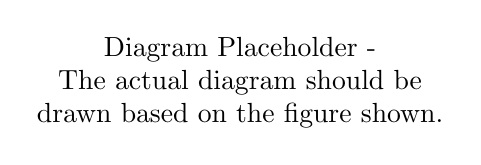
\begin{tikzpicture}
        % The diagram provided in the question was a conceptual one,
        % not suitable for replication with tikz without additional details.
        % Therefore, only a placeholder is included.
        \node at (0,0) [align=center] {Diagram Placeholder -\\ The actual diagram should be\\ drawn based on the figure shown.};
    \end{tikzpicture}
\end{center} 

\item In the graphs below, the resistance \(R\) of a superconductor is shown as a function of its temperature \(T\) for two different magnetic fields \(B_1\) (solid line) and \(B_2\) (dashed line). If \(B_2\) is larger than \(B_1\), which of the following graphs shows the correct variation of \(R\) with \(T\) in these fields?
    \begin{tasks}(2)
        \task Graph A
        \task Graph B
        \task Graph C
        \task Graph D
    \end{tasks}

\item A superconductor has \( T_c (0) = 100 K\). When a magnetic field of \(7.5\) Tesla is applied, its \(T_c\) decreases to \(75 K\). For this material one can definitely say that when
    \begin{tasks}(2)
        \task \(B = 5\) Tesla, \( T_c (B) = 80 K\)
        \task \(B = 5\) Tesla, \(75 K < T_c (B) < 100 K\)
        \task \(B = 10\) Tesla, \(75 K < T_c (B) < 100 K\)
        \task \(B = 10\) Tesla, \(T_c (B) = 70 K\)
    \end{tasks} 
